%\documentclass[aspectratio=169, handout]{beamer}
\documentclass[aspectratio=169]{beamer}


\makeatletter
\renewcommand*\env@matrix[1][\arraystretch]{%
  \edef\arraystretch{#1}%
  \hskip -\arraycolsep
  \let\@ifnextchar\new@ifnextchar
  \array{*\c@MaxMatrixCols c}}
\makeatother

\usepackage{tikz}
\usetikzlibrary{tikzmark,fit,shapes.geometric}


\newcommand{\transp}{^{\rm{T}}}

\usepackage{cases}
\usepackage[english]{babel}
% or whatever
\usepackage{xcolor}
\usepackage{colortbl}
\usepackage[latin1]{inputenc}
\usepackage[super]{nth}
% or whatever
%\setbeamertemplate{footline}[page number]
\setbeamertemplate{footline}
        {
      \leavevmode%
      \hbox{%
      \begin{beamercolorbox}[wd=.333333\paperwidth,ht=2.25ex,dp=1ex,center]{author in head/foot}%
        \usebeamerfont{author in head/foot}\insertshortauthor%~~(\insertshortinstitute)
      \end{beamercolorbox}%
      \begin{beamercolorbox}[wd=.333333\paperwidth,ht=2.25ex,dp=1ex,center]{title in head/foot}%
        \usebeamerfont{title in head/foot}\insertshorttitle
      \end{beamercolorbox}%
      \begin{beamercolorbox}[wd=.333333\paperwidth,ht=2.25ex,dp=1ex,right]{date in head/foot}%
        \usebeamerfont{date in head/foot}\insertshortdate{}\hspace*{2em} \insertframenumber{}  \hspace*{2em}%/ \inserttotalframenumber\hspace*{2ex} 

    %#turning the next line into a comment, erases the frame numbers
        

      \end{beamercolorbox}}%
      \vskip 0pt%
    }

\usepackage{times}
\usepackage[T1]{fontenc}
\usepackage{psfrag}
\usepackage{algorithm}
\usepackage{amsmath}
\usepackage{amssymb}
\usepackage{tabularx}
\usepackage{algpseudocode}
\usepackage{mathrsfs}
\usepackage{textpos}
\usepackage{graphicx}
\usepackage{tcolorbox}
\usepackage{multicol}
\usepackage{tikz}
\usetikzlibrary{arrows.meta,shapes.arrows}
%\setkeys{Gin}{draft}
\usepackage{caption}
\captionsetup{font=scriptsize,labelfont=scriptsize}
\usepackage{color}
\DeclareCaptionFont{blue}{\color{blue}}
\captionsetup{labelfont=blue}
\usepackage{tikz}
\tikzset{
  every overlay node/.style={
    draw=white,anchor=north west,
  },
}
\def\checkmark{\tikz\fill[scale=0.4](0,.35) -- (.25,0) -- (1,.7) -- (.25,.15) -- cycle;}
\def\tikzoverlay{%
   \tikz[baseline,overlay]\node[every overlay node]
}%
%\DeclareGraphicsRule{.png}{png}{.png.bb}{}

\newtheorem{assumption}{Assumption} %jw

\newcommand{\T}{{\rm T}}

\newcommand\blfootnote[1]{%
  \begingroup
  \renewcommand\thefootnote{}\footnote{#1}%
  \addtocounter{footnote}{-1}%
  \endgroup
}
\setcounter{tocdepth}{1}
\beamertemplatenavigationsymbolsempty


\title[Lecture 9: Regression] % (optional, use only with long paper titles)
{Data, Environment and Society: \\{Lecture 9: Intro to regression}}


%\subtitle
%{Include Only If Paper Has a Subtitle}

\author[ER190C: Data, Environment and Society] 
{Instructor: Duncan Callaway\\
GSI: Seigi Karasaki} 
% - Give the names in the same order as the appear in the paper.
% - Use the \inst{?} command only if the authors have different
%   affiliation.

%\logo{
%\includegraphics[width=1.5cm,height=1.5cm,keepaspectratio]{uvic_logo_h.jpg}
%}
\vspace{-20mm}
\institute[UC Berkeley] % (optional, but mostly needed)
 {\small{ \bf September 20, 2018}}


\date[September 20, 2018]


\begin{document}

\begin{frame}[plain, noframenumbering]
  \titlepage
\end{frame}

\begin{frame}{Announcements}

\textbf{Today}
\begin{itemize}
\item Review bias-variance tradeoff
\item Regression
\begin{itemize}
	\item K-nearest neighbors
	\item Linear least squares
\end{itemize}
\end{itemize}

\textbf{Reading}
\begin{itemize}
\item Today's lecture draws from DS100 Ch10, ISLR Ch 2, ISLR Ch 3.1
\item For next week
\begin{itemize}
\item Read Alstone \textit{et al} for next Tuesday -- in class discussion
\item Review ISLR Ch 3.1-3.2
\end{itemize}
\end{itemize}

\end{frame}

\begin{frame}{(review) Error or residual?}

\begin{eqnarray*}
y_i = f(x_i) + \epsilon_i & \text{ the ``true'' model, if one exists. }\\
y_i = \hat{f}(x_i) + e_i & \text{ the relationship between the data and the estimate. }
\end{eqnarray*}

\hspace{5mm}

\pause
So:
\begin{eqnarray*}
\epsilon_i&\text{variation in $y$ that is uncorrelated with $x$.}\\
e_i = y_i - \hat{f}(x_i) & \text{ the ``residual'' between the data and the estimate. }
\end{eqnarray*}

\end{frame}

\begin{frame}{(Review) How to evaluate how well a model performs?}

Generic term: the \textit{Cost function.}

\begin{itemize}
\item Cost functions can be used to describe how much of the variation in the data can be captured by the model.
\item Example: The mean squared error:

\begin{align*}
MSE &= \frac{1}{n} ((y_1 - \hat{y}_1)^2 + (y_2 - \hat{y}_2)^2 + \cdots + (y_n - \hat{y}_n)^2) \\\\
 \onslide<2->{&= \frac{1}{n} (e_1^2 + e_2^2 + \cdots + e_n^2)} \\
 \onslide<3->{&=\frac{1}{n} \sum_{i=1}^n e_i^2}
\end{align*}
\end{itemize}

\end{frame}


\begin{frame}{(Review) A thought experiment from ISLR Ch 2}

\begin{columns}
\column{0.5\textwidth}
Suppose you have four different model forms to choose from.  When you fit them to the data, you get this figure.

\vspace{5mm}

Which model should you choose?  
\begin{itemize}
\item The one that minimizes mean squared error?
\item Careful!  Doesn't the squiggly one minimize mean squared error?
\item To do model selection we need to understand the concept of training and testing data.
\end{itemize}

\column{0.5\textwidth}
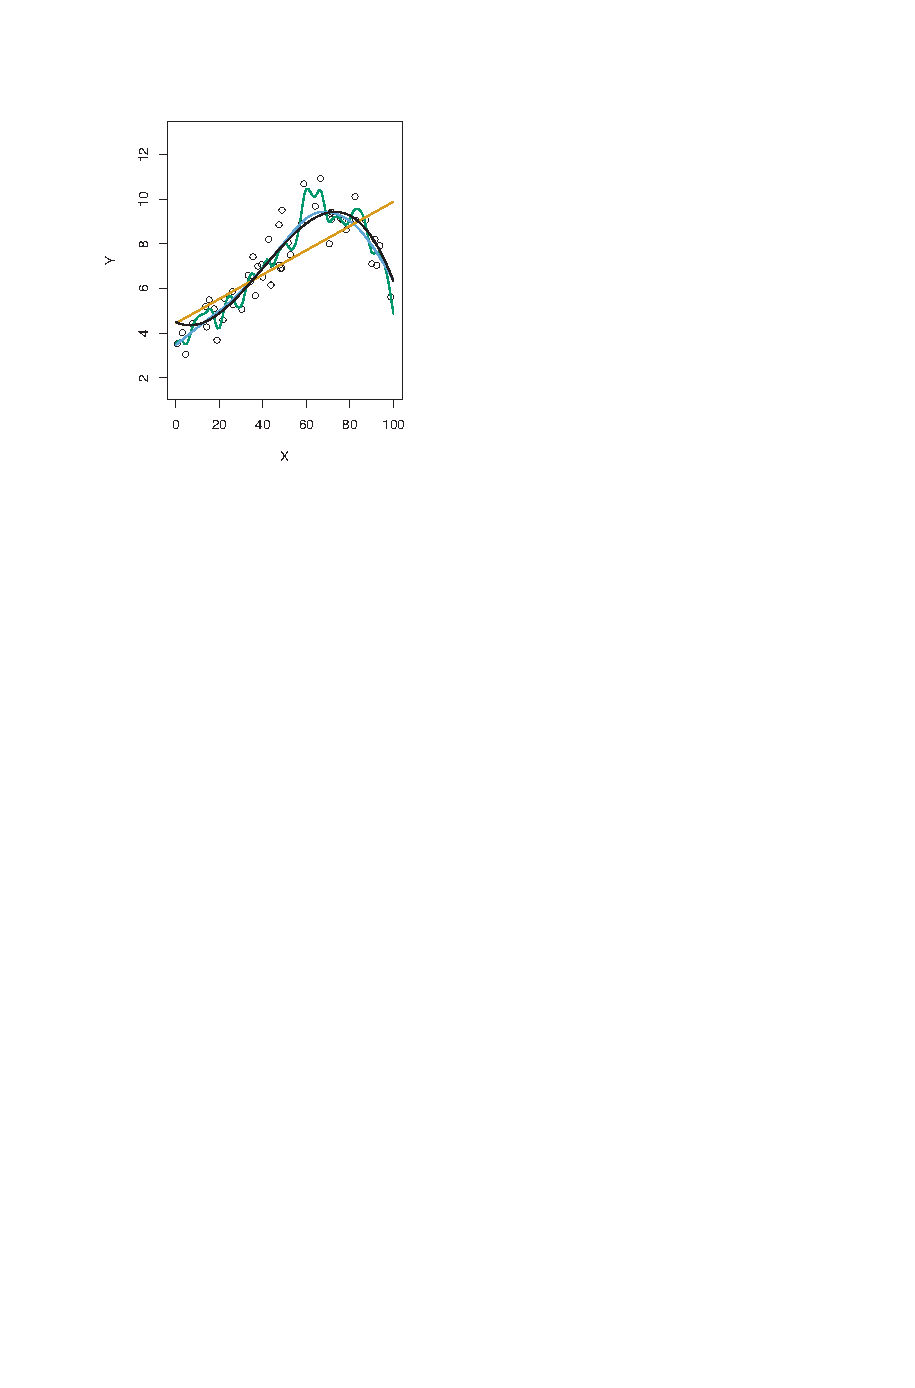
\includegraphics[scale=1]{figures/islr2_9a.pdf}
\end{columns}

\end{frame}

\begin{frame}{(Review) Concept:  Test and training data}


\begin{columns}
\column{0.65\textwidth}


Choosing between different models can be done by partitioning your data in to ``training'' and ``test'' data.

\begin{itemize}
\item ``Training data'': The data we use to choose the parameters of an individual model. 

\hspace{5mm}

\item ``Test data'': A set of data we withhold; it's not for training.  We use this data set to compare how different \textit{models} perform relative to one another.  

\end{itemize}
\column{0.35\textwidth}

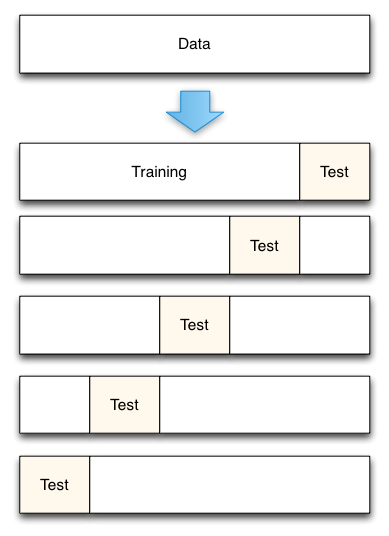
\includegraphics[scale=0.35]{figures/07_cross_validation_diagram}
\begin{tiny}
Source: kaggle.com
\end{tiny}
\end{columns}


\end{frame}


\begin{frame}{(Review) MSE for test and training data}


\begin{columns}
\column{0.5\textwidth}


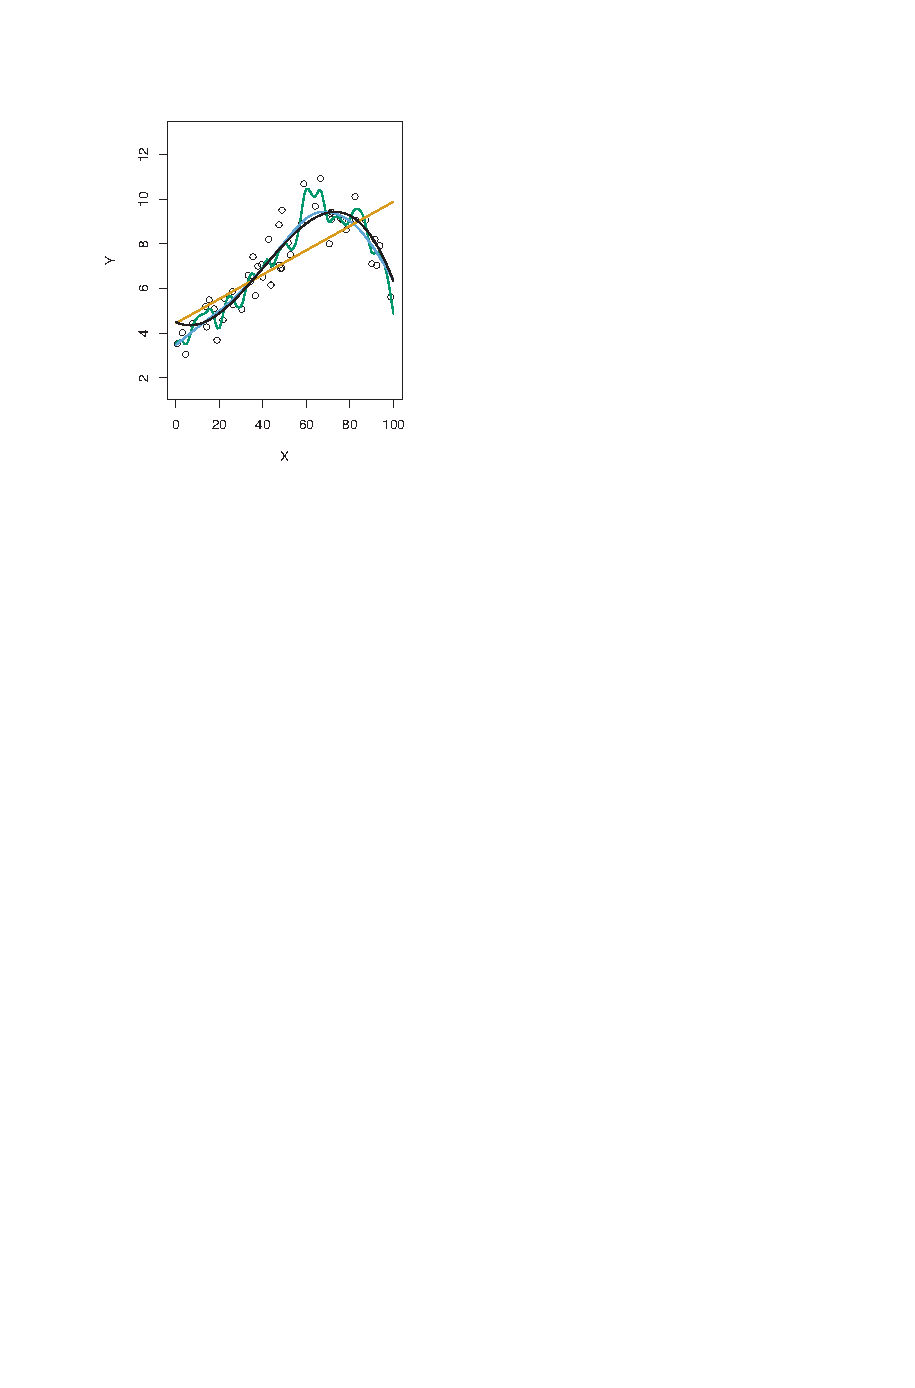
\includegraphics[scale=1]{figures/islr2_9a.pdf}


What might a plot of MSE versus model ``flexibility'' look like?


\column{0.5\textwidth}

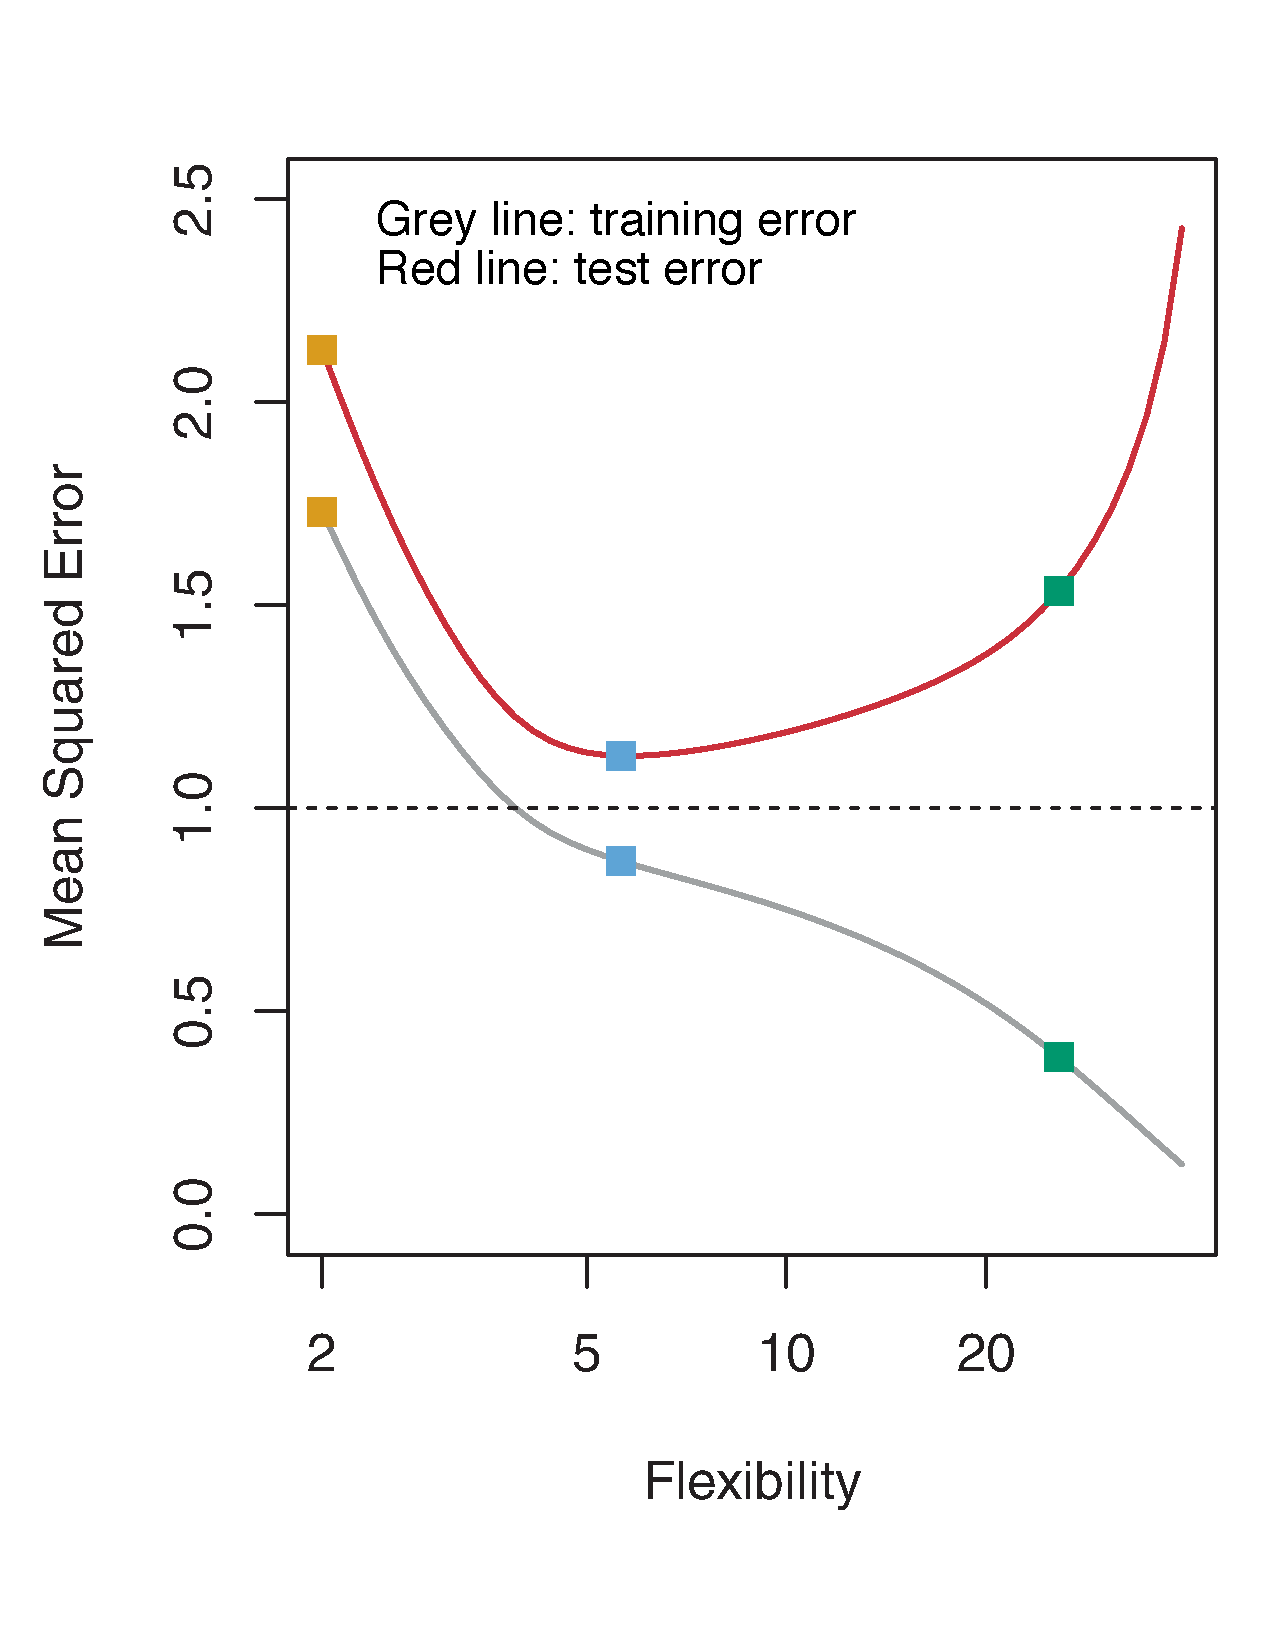
\includegraphics[scale=0.25]{figures/islr2_9b.pdf}
\end{columns}


\end{frame}


\begin{frame}{Bias v. Variance}

\textbf{Bias}: 
\begin{itemize}
\item The propensity for a model to produce errors that are systematically high or low
\item Bias can be positive in one range of the predictor and negative in another.  
\end{itemize}


\textbf{Variance}
\begin{itemize}
\item The propensity for a model to make very different predictions if it is fit with two different training data sets that are sampled from the same population.
\end{itemize}

\hspace{5mm}

Total error can be decomposed:

\begin{align*}
\text{Avg }(y_0-\hat{f}(x_0))^2 = & \text{(variance in a prediction, across different training data)}\\
&+(\text{systematic bias})^2 + \text{(variance in }y\text{ that's uncorrelated with }x)\\
\onslide<2->{ =  &\text{var} (\hat{f}(x_0)) + [\text{bias}(\hat{f}(x_0))]^2+\text{var}(\epsilon_0)}
\end{align*}

\end{frame}


\begin{frame}{Bias v. Variance, ctd.}


\begin{columns}
\column{0.4\textwidth}

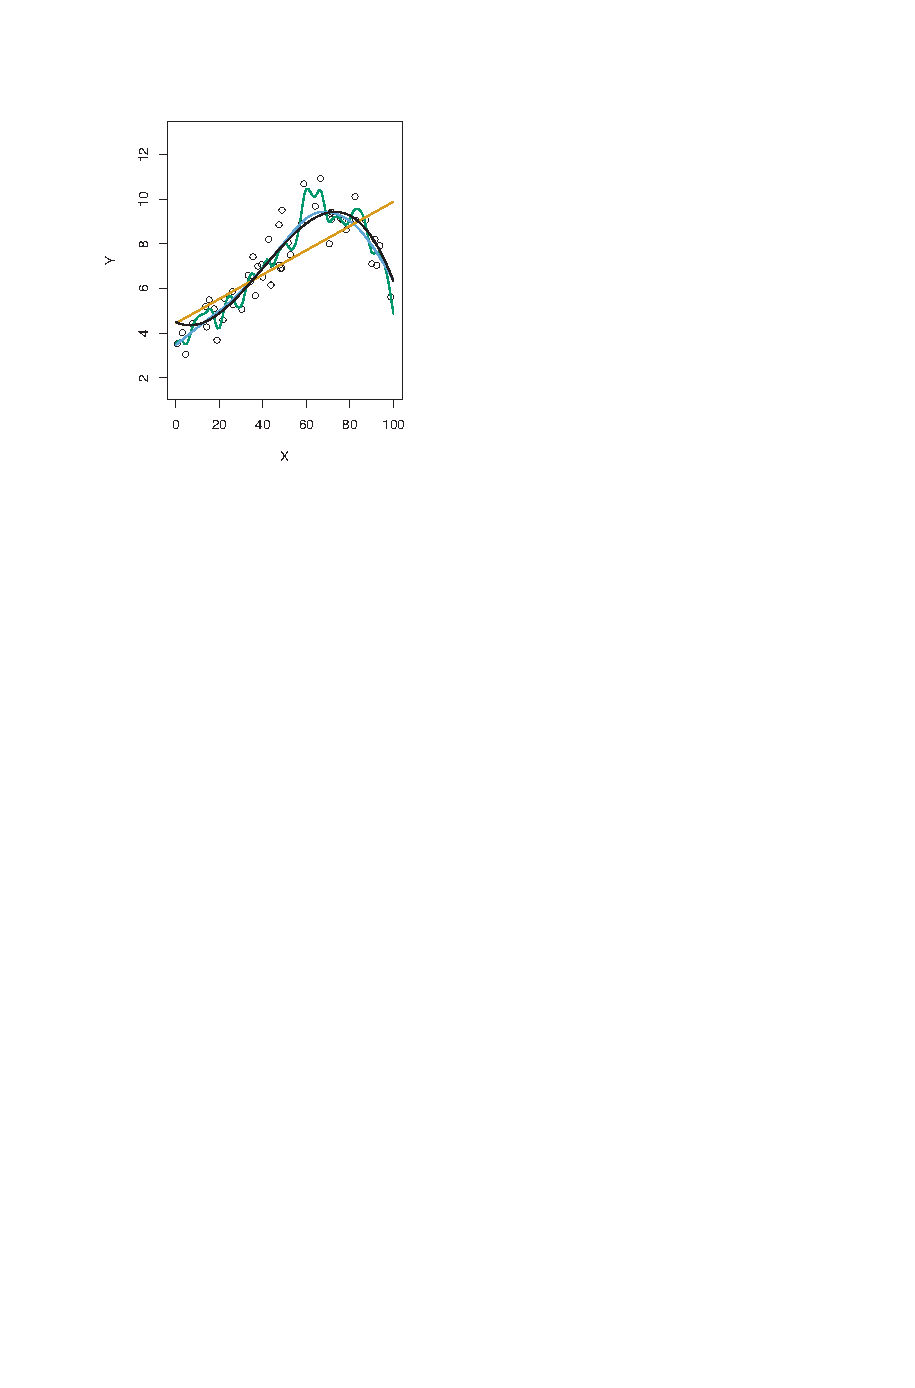
\includegraphics[scale=1]{figures/islr2_9a.pdf}

\column{0.6\textwidth}

Which model has the greatest propensity for bias?
\begin{itemize}
\item<2-> The linear one.  In ranges of $x$, it systematically under- or over-estimates. 
\end{itemize}

\hspace{5mm}

Which model has the greatest propensity for variance?
\begin{itemize}
\item<3-> The squiggly one.  If we drew another sample of data, we'd probably get very different squiggles.
\end{itemize}
\end{columns}



\end{frame}

\begin{frame}{Decomposing bias-variance}

\begin{columns}
\column{0.375\textwidth}
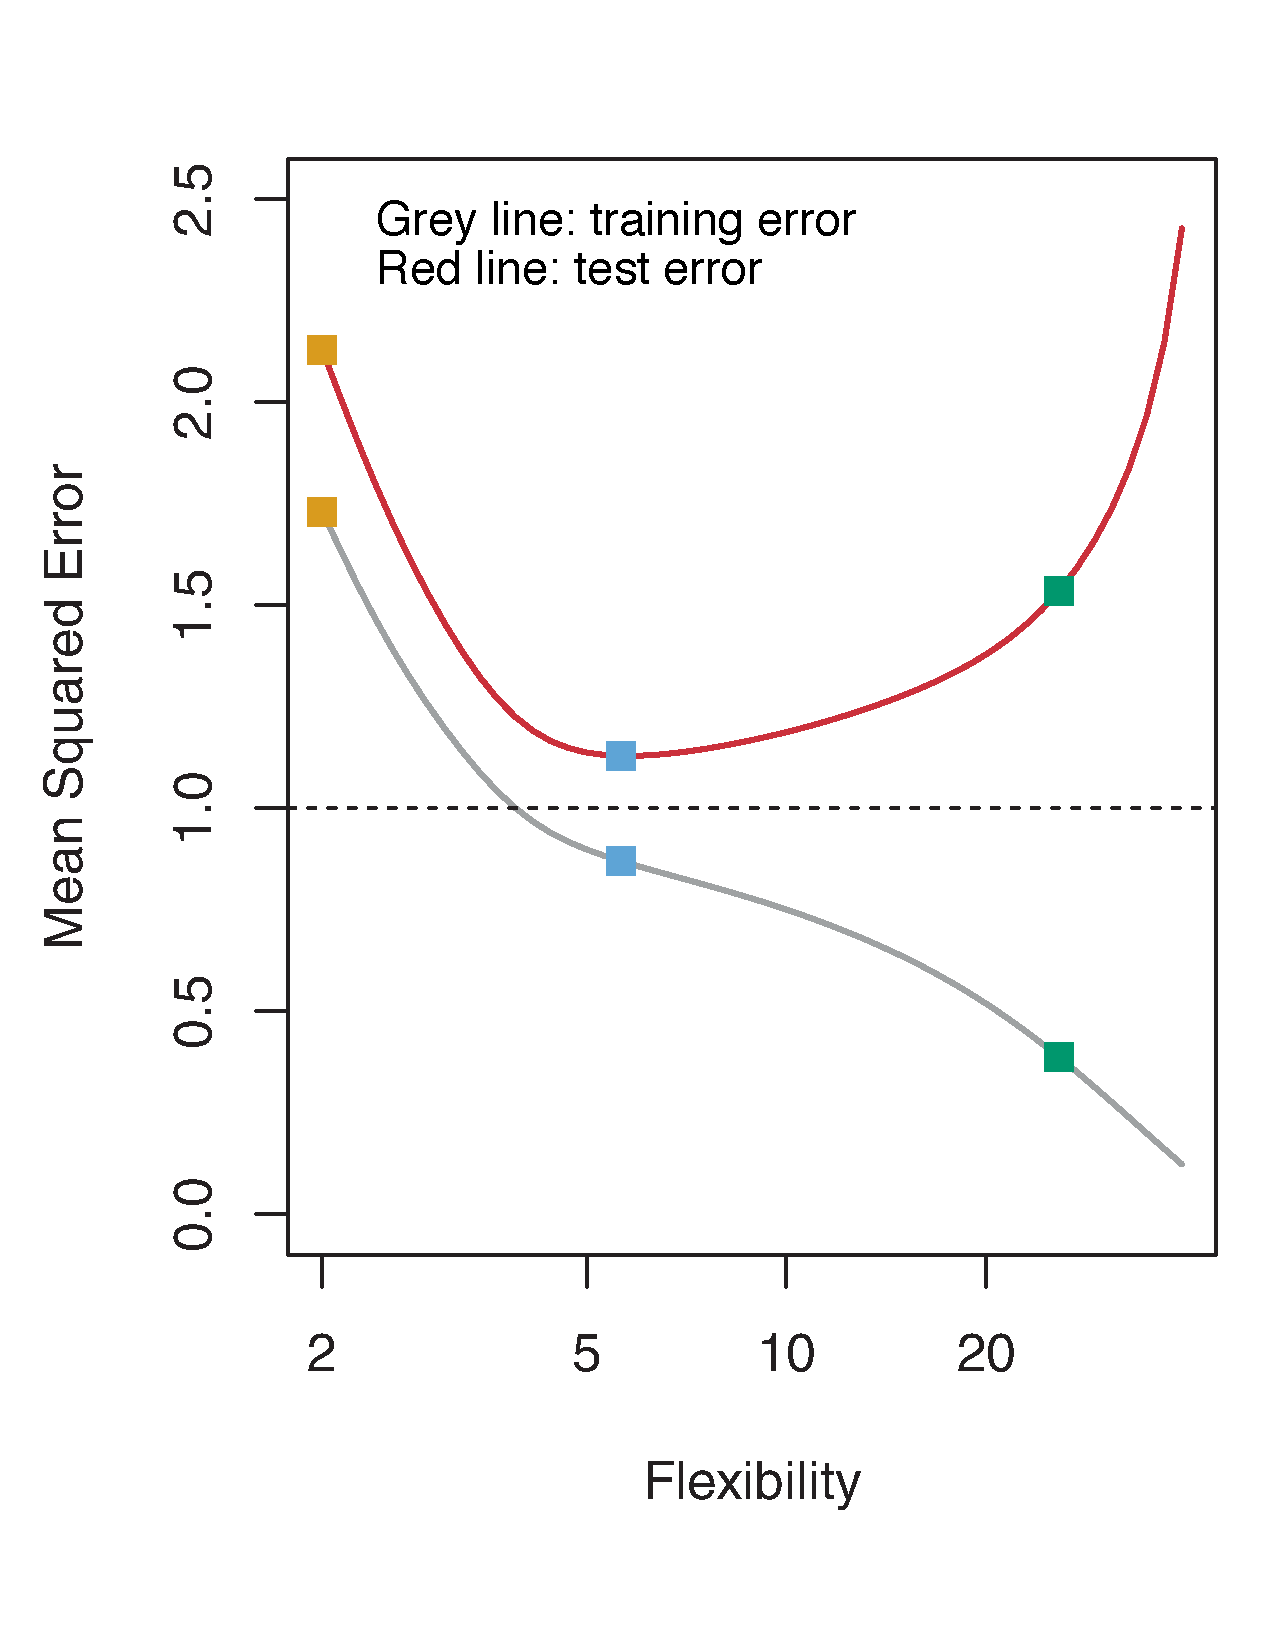
\includegraphics[scale=0.25]{figures/islr2_9b.pdf}

\column{0.3\textwidth}
Take a moment to think about how bias and variance add up to make the red curve on the left.  Try to draw bias and variance separately.  

\column{0.3\textwidth}
\pause 
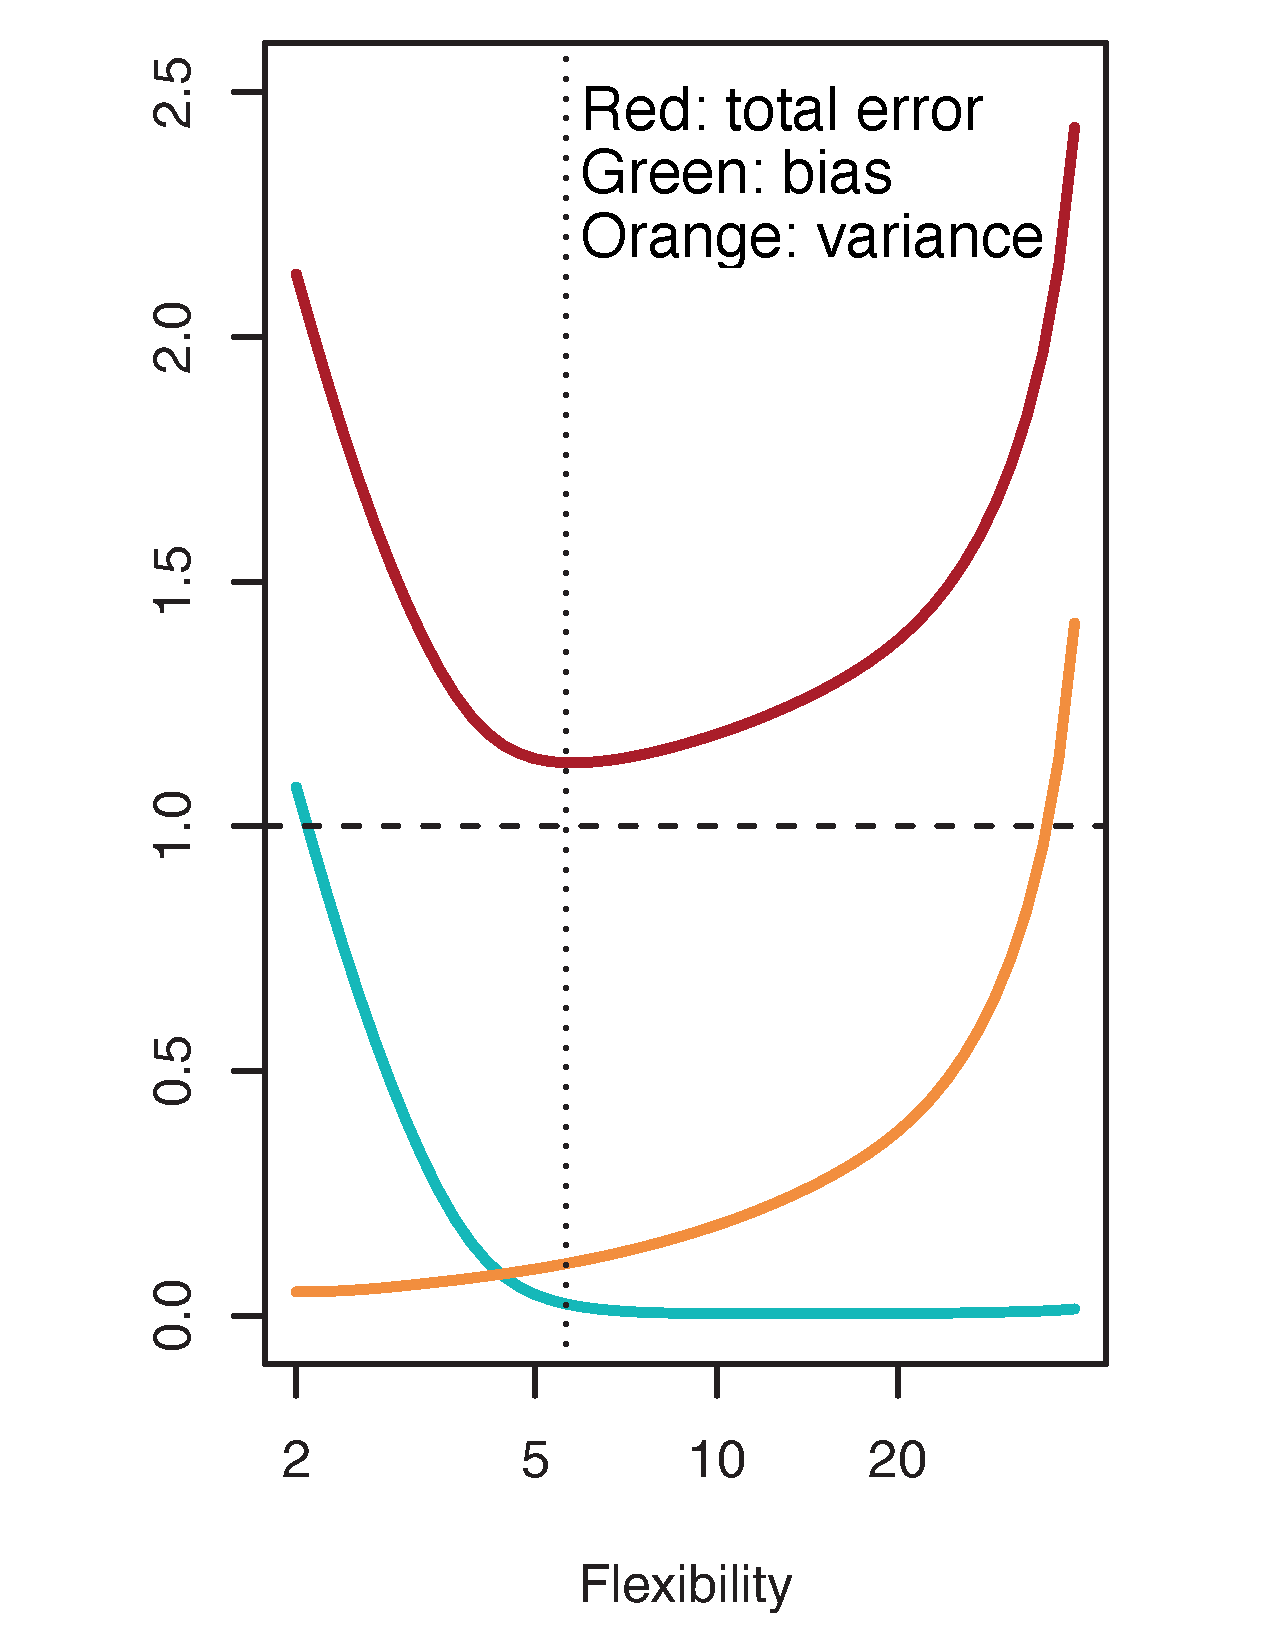
\includegraphics[scale=0.21]{figures/islr2_12a_text.pdf}

\end{columns}

\end{frame}

\begin{frame}{Parametric vs. non-parametric models}

The model examples we discussed Tuesday were \textbf{parametric}, meaning they relate inputs to outputs with a mathematical function defined by parameters.  

\vspace{5mm}

But \textbf{non-parametric} models are also possible.  
\begin{itemize}
\item These don't use functions with coefficients
\item Instead the data \textit{become} the model
\end{itemize}

\vspace{5mm}

It's easiest to see this by example using the K-nearest neighbors algorithm.

\end{frame}

\begin{frame}{K-nearest neighbors (KNN)}

 We'll work with just a one-dimensional independent variable. For example, 
\begin{itemize}
\item $y_i$ could be NOx emissions from a power plant, 
\item $x_i$ could be its coal use; 
\item different $i$ would correspond to different power plants in different years.
\end{itemize}

\vspace{5mm}
Definitions:
\begin{itemize}
\item First, define proximity between two points as $|x_i-x_j|$
\item Next, define $\mathcal{N}_i$ as the set of $K$ points closest to $x_i$ 
\end{itemize}

\end{frame}

\begin{frame}{K-nearest neighbors}
The basic idea behind using KNN for regression (i.e. predicting a continuous variable or set of variables) is simple:

\begin{align*}
\hat{y}_j = \frac{1}{K} \sum_{i\in \mathcal{N}_j} y_i
\end{align*}

In other words, the prediction equals the average of the $K$ nearest points.
\end{frame}

\begin{frame}{If you're working with KNN, what is your most important decision?}

\pause

\begin{center}
What is $K$?
\end{center}

Check of intuition:  Would increasing $K$ reduce or increase bias?\pause \textbf{  Increase!}

\begin{itemize}
\item Using a lower $K$ would cause the estimates to more closely follow the underlying data.  
\item In the extreme, $K=1$ would make the model equal the underlying data.
\item At the other extreme, $K=n$ would make the model equal the sample mean.
\end{itemize}
\end{frame}


\begin{frame}{Linear regression}

\textbf{Regression:} A method to estimate the expected value of an output variable ($y$), \textit{conditional} on one or more input values ($x$)

\begin{itemize}
\item KNN regression does this by averaging nearby values.

\item Linear regression does this by fitting a linear function to the data.

\item Broadly speaking, \textit{regression} can be used for prediction.

\item \textit{Linear} regression specifically can also be used for inference.

\item Many of the methods we'll work with later in the semester will be rooted in linear regression.
\end{itemize}

\end{frame}

\begin{frame}{The basic model}

\begin{itemize}
\item $x_i$: one dimensional independent variable 
\item $y_i$: one dimensional dependent variable
\end{itemize}

\begin{align*}
y_i &= \hat{\beta}_0 + \hat{\beta}_1 x_i + e_i\\
\hat{y_i} &= \hat{\beta}_0 + \hat{\beta}_1 x_i
\end{align*}

\begin{itemize}
\item We use the $\hat{\cdot}$ symbol to denote an estimate, or prediction
\end{itemize}
\end{frame}


\begin{frame}{(extremely important) Side note: Optimality.}


Define the ``argument'' that minimizes a function $f$ with respect to $\theta$ as:

\begin{align*}
\theta^* = \arg \min_{\theta} f(\theta)
\end{align*}

In the plot below, what's $\theta^*$?

\vspace{-8mm}

\begin{columns}
\column{0.5\textwidth}
\begin{center}
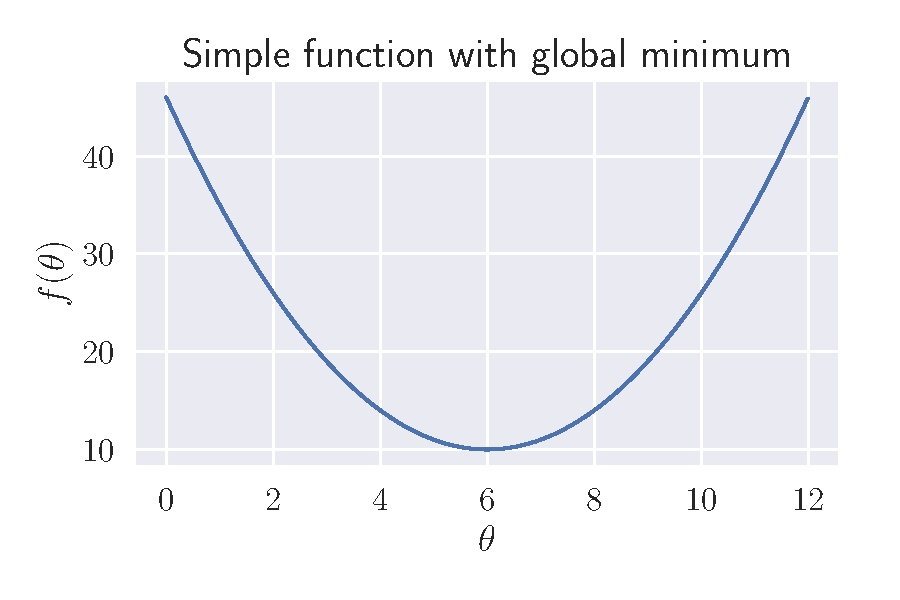
\includegraphics[scale=0.5]{simple_min}
\end{center}

\column{0.5\textwidth}
\pause
\begin{align*}
\theta^* = \arg \min_{\theta} f(\theta) = 6\\
\pause
f(\theta^*) =10
\end{align*}

\end{columns}

\end{frame}

\begin{frame}{What do the minima share in common?}

\begin{columns}
\column{0.5\textwidth}
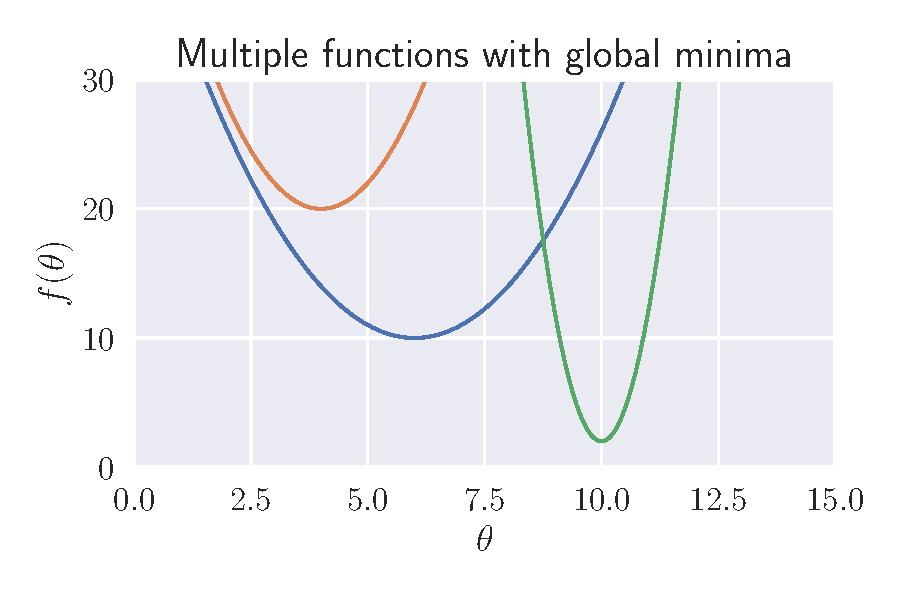
\includegraphics[scale=0.5]{multiple_min}

\column{0.5\textwidth}
\pause
\begin{align*}
\frac{\partial f(\theta)}{\partial \theta}\Big|_{\theta^*} = 0
\end{align*}

\end{columns}
\end{frame}


\begin{frame}{What's the challenge here?}

\begin{columns}
\column{0.5\textwidth}
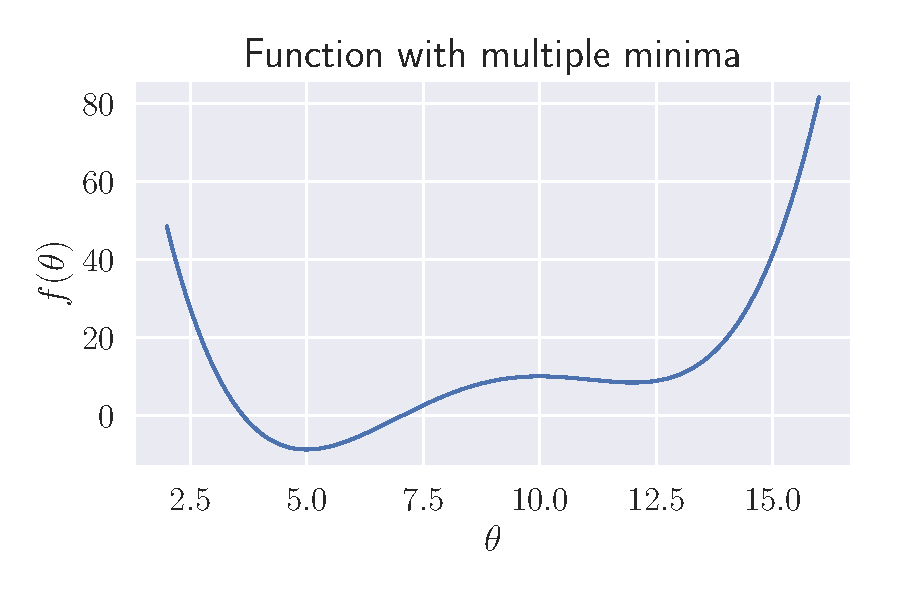
\includegraphics[scale=0.5]{multiple_extrema}

\column{0.5\textwidth}
\pause
$\frac{\partial f(\theta)}{\partial \theta} = 0$ at more than one point.  

\vspace{5mm}

The function is said to be ``non-convex''

\vspace{5mm}

\pause
Which should we choose?

\begin{itemize}
\item We could enumerate all the solutions and choose the best.  
\pause
\item But that can get really tedious with complicated functions.
\end{itemize}

\end{columns}
\end{frame}


\begin{frame}{Estimation can be framed as an optimization problem}

In many forms of estimation, we set up the problem as follows:

\begin{align*}
\{\hat{\beta}_0, \hat{\beta}_1\} &= \arg \min_{\beta_0,\beta_1} J(\beta_0,\beta_1)
\end{align*}

...where $\beta$s are the parameters we wish to identify.  

\vspace{5mm}

In this course, we'll be looking at a broad variety of ways to define the \textit{cost function}, $J$.

\end{frame}

\begin{frame}{Linear regression as optimization}

In ``least squares'' linear regression, the starting point for estimation is

\begin{align*}
\{\hat{\beta}_0, \hat{\beta}_1\} &= \arg \min_{\beta_0,\beta_1} \sum_{i=1}^n (e_i)^2\\
\onslide<2->{&= \arg \min_{\beta_0,\beta_1} \sum_{i=1}^n (y_i - \hat{y}_i)^2}\\
\onslide<3->{&= \arg \min_{\beta_0,\beta_1} \sum_{i=1}^n (y_i - (\beta_0 + \beta_1 x_i))^2}\\
\end{align*}
\end{frame}

\begin{frame}{Why choose a quadratic (squared) objective function?}

\pause
Hint: 

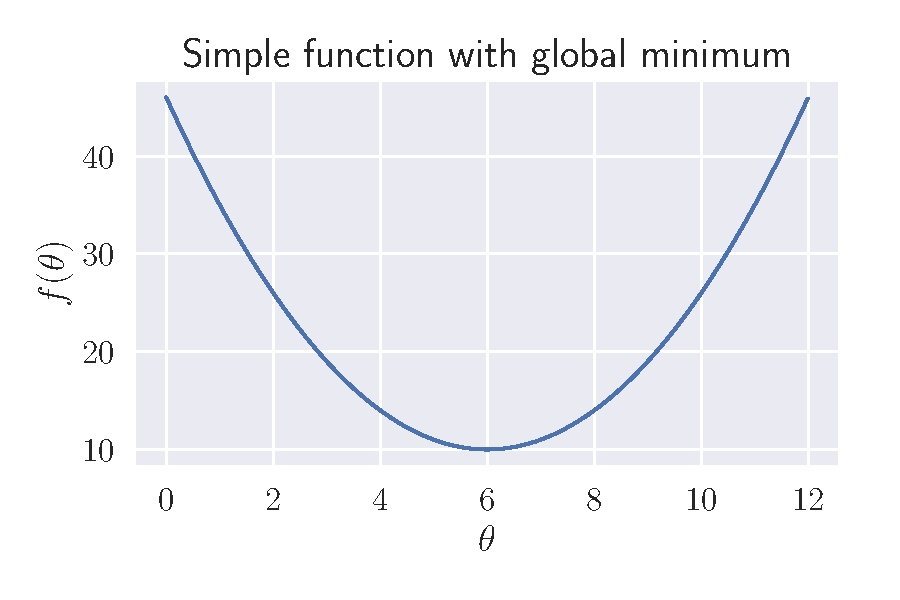
\includegraphics[width=0.5\textwidth]{simple_min}
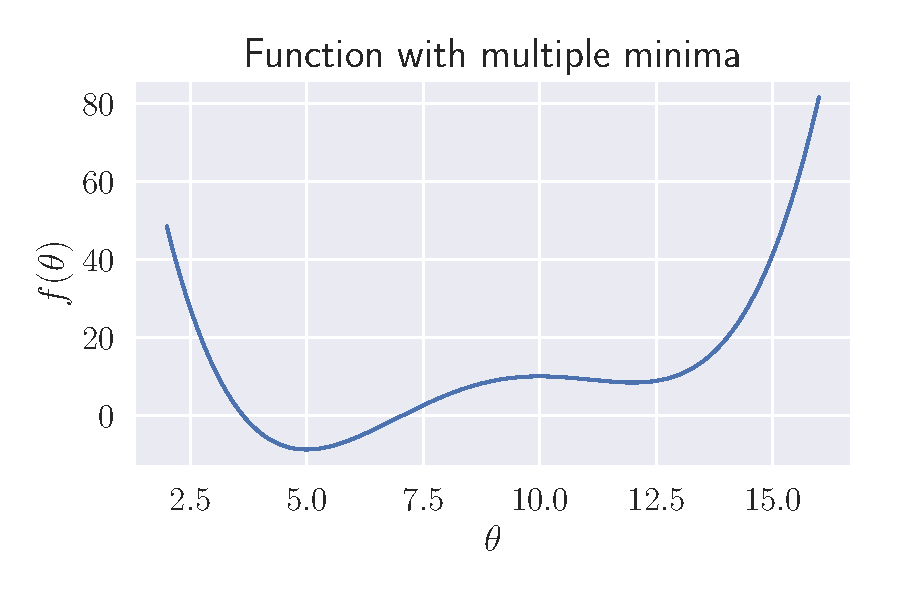
\includegraphics[width=0.5\textwidth]{multiple_extrema}

\pause

With least squares, the cost function
\begin{itemize}
\item Has one global minimum
\item Is differentiable -- we can write an equation for 
$\frac{\partial f(\theta)}{\partial \theta} = 0$
\end{itemize}

\end{frame}

\begin{frame}{Solving the estimation problem}

\begin{align*}
\{\hat{\beta}_0, \hat{\beta}_1\} &= \arg \min_{\beta_0,\beta_1} \sum_{i=1}^n (y_i - (\beta_0 + \beta_1 x_i))^2
\end{align*}

So the optimal parameters must satisfy:


\begin{align*}
\frac{\partial \sum_{i=1}^n (y_i - (\beta_0 + \beta_1 x_i))^2}{\partial \beta_0} &= 0\\\\
\frac{\partial  \sum_{i=1}^n(y_i - (\beta_0 + \beta_1 x_i))^2}{\partial \beta_1} &= 0
\end{align*}
\end{frame}

\begin{frame}{The solution: }

\begin{align*}
\frac{\partial  \sum_{i=1}^n(y_i - (\hat{\beta}_0 + \hat{\beta}_1 x_i))^2}{\partial \hat{\beta}_0} = 0 \quad\quad &\Rightarrow \hat{\beta}_0  =\bar{y} - \hat{\beta}_1\bar{x}\\\\
\frac{\partial   \sum_{i=1}^n(y_i - (\hat{\beta}_0 + \hat{\beta}_1 x_i))^2}{\partial \hat{\beta}_0} = 0 \quad\quad &\Rightarrow 
\hat{\beta}_1 = \frac{ \sum_{i=1}^n(x_i-\bar{x})(y_i-\bar{y})}{\sum_{i=1}^n (x_i-\bar{x})^2}
\end{align*}

\end{frame}

\begin{frame}{Before moving on, a little linear algebra:}

Here are two vectors:  
\begin{align*}
\mathbf{a} =  
\begin{bmatrix} 
	a_1 \\
	a_2  
\end{bmatrix}\\
\mathbf{b}=
 \begin{bmatrix}
	b_1\\
	b_2
\end{bmatrix} 
\end{align*}

Then the ``dot'' product of the two vectors is

\begin{align*}
\mathbf{a}\cdot \mathbf{b} = a_1b_1 + a_2b_2
\end{align*}

\end{frame}


\begin{frame}{Next, a little more linear algebra:}

We can also multiply \textit{matrices} and vectors.  Matrices are like column vectors stacked side by side
\begin{align*}
\mathbf{A} =  
\begin{bmatrix} 
	a_{11} &a_{12}\\
	a_{21} &a_{22}
\end{bmatrix}
\end{align*}

Then matrix multiplication gives us
\begin{align*}
\mathbf{A}\mathbf{b} = 
\begin{bmatrix} 
	a_{11} &a_{12}\\
	a_{21} &a_{22}
\end{bmatrix}
\begin{bmatrix}
	b_1\\
	b_2
\end{bmatrix} 
=\begin{bmatrix}
	a_{11}b_1+a_{12}b_2 \\
	a_{21}b_1+a_{22}b_2  
\end{bmatrix} 
\end{align*}

\pause
Each element of the resulting matrix (or vector) is the dot product of a row of the first term ($\mathbf{A}$) and a column of the second ($\mathbf{b}$)

\vspace{5mm}
Therefore:   the horizontal ``dimension'' of the first must be the same as the vertical ``dimension'' of the second.

\end{frame}

\begin{frame}{Let's define matrices for our data:}


Suppose we have $n$ observations, $(x_i, y_i)$.  We'll arrange them all into a matrix form:

\begin{align*}
X = \begin{bmatrix} 
  1 & x_1\\
  1 & x_2\\
  \vdots & \vdots \\
  1 & x_n 
\end{bmatrix}, 
Y = 
\begin{bmatrix} 
  y_1\\
  y_2\\
   \vdots \\
  y_n 
\end{bmatrix} 
\end{align*}

Note: when we start working with more than one independent variable, $X$ will have a new column for each new variable.  

\end{frame}

\begin{frame}{And then a lot more linear algebra:}
Let's define the `transpose':
\begin{align*}
X = \begin{bmatrix} 
  1 & x_1\\
  1 & x_2\\
  \vdots & \vdots \\
  1 & x_n 
\end{bmatrix} \quad \Rightarrow \quad X^T = \begin{bmatrix} 
  1 & 1&\ldots & 1\\
  x_1& x_2 &\ldots & x_n
\end{bmatrix} 
\end{align*}

\pause

Now a challenge question: what's the product of these two matrices:
\begin{align*}
X^TX = 
\begin{bmatrix} 
  1 & 1&\ldots & 1\\
  x_1& x_2 &\ldots & x_n
\end{bmatrix} 
\begin{bmatrix} 
  1 & x_1\\
  1 & x_2\\
  \vdots & \vdots \\
  1 & x_n 
\end{bmatrix}
\end{align*}

\end{frame}

\begin{frame}{Product of a matrix and its transpose}

\begin{align*}
X^TX &= 
\begin{bmatrix} 
  1 & 1&\ldots & 1\\
  x_1& x_2 &\ldots & x_n
\end{bmatrix} 
\begin{bmatrix} 
  1 & x_1\\
  1 & x_2\\
  \vdots & \vdots \\
  1 & x_n 
\end{bmatrix}\\\\
\onslide<2->{&=
\begin{bmatrix}[1.4]
	\text{1st row dot 1st col} & \text{1st row dot 2nd col}   \\
	\text{2nd row dot 1st col} & \text{2nd row dot 2nd col} 
\end{bmatrix}}\\\\
\onslide<3->{&=
\begin{bmatrix}[1.4]
	\sum_{i=1}^n 1\cdot 1 & \sum_{i=1}^n 1\cdot x_i   \\
	\sum_{i=1}^n 1\cdot x_i & \sum_{i=1}^n x_i\cdot x_i 
\end{bmatrix}}
\onslide<4->{\quad=
\begin{bmatrix}[1.4]
	n & n  \bar{x}  \\
	n\bar{x} & \sum_{i=1}^n x_i^2 
\end{bmatrix}}
\end{align*}
\end{frame}


\begin{frame}{Doing linear algebra in numpy:}

See the in-class workbook!

\end{frame}


\begin{frame}{Finally, the ``normal equations''}

We showed a  way to compute $\beta$ coefficients individually a few slides ago.

\vspace{5mm}\pause

However that can get tedious if you're doing \textit{multiple} linear regression -- i.e. if you have more than one independent variable.  

\vspace{5mm}

The so-called ``normal equations'' give a nice, compact form to get the parameters.

\begin{align*}
\Theta &= 
\begin{bmatrix}
	\beta_0\\
	\beta_1
\end{bmatrix}
= 
(X^TX)^{-1}X^TY\\
&= 
\left(
\begin{bmatrix} 
  1 & 1&\ldots & 1\\
  x_1& x_2 &\ldots & x_n
\end{bmatrix} 
\begin{bmatrix} 
  1 & x_1\\
  1 & x_2\\
  \vdots & \vdots \\
  1 & x_n 
\end{bmatrix} \right)^{-1}
\begin{bmatrix} 
  1 & 1&\ldots & 1\\
  x_1& x_2 &\ldots & x_n
\end{bmatrix} 
\begin{bmatrix} 
  y_1\\
  y_2\\
   \vdots \\
  y_n 
\end{bmatrix} 
\end{align*}
\end{frame}

\begin{frame}{A note for computing and linear algebra geeks}

The normal equations are an efficient way to solve the least squares linear regression problem \textit{when the number of independent variables is relatively small.}

\vspace{5mm}

But!  Inverting a matrix (the $(\cdot)^{-1}$ part) is a heavy computational lift -- especially as the size of the matrix gets big. 


\vspace{5mm}

Later in the semester we'll talk about an alternative approach, called ``gradient descent'', 
\begin{itemize}
\item  It searches for the optimal point on the cost function in a more manual way. 
\item But it's actually faster than getting the solution using the normal equations.
\end{itemize}
\end{frame}

\end{document}


